% title: Fill preserves context and replaces specifications
% description: The topic context remains unchanged. The answer Str specification becomes text and the score Float specification becomes a number, in the same dictionary structure.
\documentclass[tikz,border=5pt]{standalone}
\usetikzlibrary{arrows.meta,calc,shapes.geometric}
\definecolor{numeric}{HTML}{4477AA}
\definecolor{textual}{HTML}{AA4499}

\tikzset{
    box/.style={draw, line width=0.8pt, minimum height=0.8cm,
                minimum width=1.8cm, inner sep=6pt, align=center},
    ir/.style={box},
    flow/.style={-{Stealth[length=5pt]}, line width=0.9pt},
    feedback/.style={flow, dashed},
    note/.style={font=\small, align=center},
    choice/.style={diamond, draw, line width=0.8pt,
                   aspect=2, inner sep=2pt, align=center},
}

\newcommand{\irframe}[2]{
    \draw[line width=0.8pt] #1 rectangle #2;
}

\newcommand{\transformarrow}[4][above]{
    \draw[flow] (#2) -- node[#1=6pt,note] {#4} (#3);
}

\begin{document}
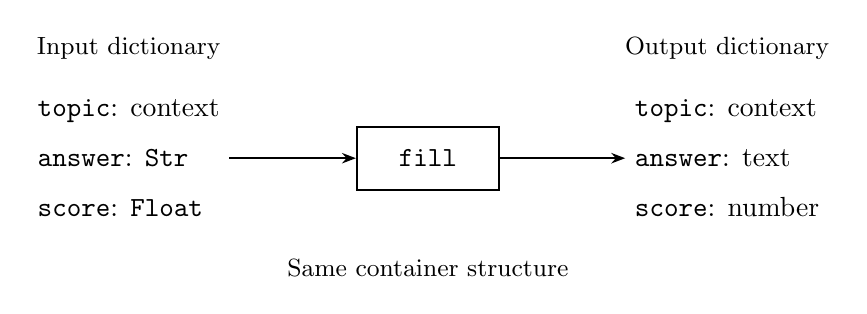
\begin{tikzpicture}

    \node[align=left] (input) at (0,0) {
        \texttt{topic}: context\\[6pt]
        \texttt{answer}: \texttt{Str}\\[6pt]
        \texttt{score}: \texttt{Float}};
    \node[box] (fill) at (3.8,0) {\texttt{fill}};
    \node[align=left] (output) at (7.6,0) {
        \texttt{topic}: context\\[6pt]
        \texttt{answer}: text\\[6pt]
        \texttt{score}: number};
    \node[note] at (0,1.4) {Input dictionary};
    \node[note] at (7.6,1.4) {Output dictionary};
    \draw[flow] (input.east) -- (fill.west);
    \draw[flow] (fill.east) -- (output.west);
    \node[note] at (3.8,-1.4) {Same container structure};

\end{tikzpicture}
\end{document}
